\section{Auswertung}
\label{sec:Auswertung}

\begin{table}[!htp]
  \begin{minipage}{0.5\linewidth}
  \centering
  \begin{tabular}{
    S[table-format=2.2]
    S[table-format=1.2]
  }
    \toprule
    {$t_{hoch}\left[\unit{\s}\right]$} & {$t_{runter}\left[\unit{\s}\right]$}\\
    \midrule
    13.85 & 12.97\\
    12.97 & 13.10\\
    13.00 & 12.85\\
    13.00 & 12.94\\
    13.00 & 13.13\\
    13.07 & 13.00\\
    13.05 & 13.03\\
    12.97 & 13.12\\
    13.03 & 13.12\\
    \bottomrule
  \end{tabular}
  \vspace{5pt}
  \caption{Fallzeiten der kleinen\\ Kugel bei Raumtemperatur}
  \label{tabellekk}
  \end{minipage}
  \begin{minipage}{0.5\linewidth}
    \centering
    \begin{tabular}{|c|c|}
      \hline
      {$t_{hoch}\left[\unit{\s}\right]$} & {$t_{runter}\left[\unit{\s}\right]$}\\
      \hline    
      52.53 & 52.78\\
      53.19 & 52.38\\
      53.79 & 52.97\\
      53.53 & 53.19\\
      \hline
    \end{tabular}
    \vspace{5pt}
    \label{tabellegk}
    \caption{Fallzeiten der großen\\ Kugel bei Raumtemperatur}
  \end{minipage}
\end{table}

\begin{table}[!htp]
  \centering
  \begin{tabular}{|c|c|c|}
    \hline
    $T [\unit{\degreeCelsius}]$ & $t_{runter} [\unit{\second}]$ & $t_{hoch} [\unit{\second}]$\\
  \end{tabular}
  \label{tabellegkt}
  \caption{Fallzeiten der großen Kugel bei steigender Temperatur}
\end{table}

%\begin{figure}
%  \centering
%  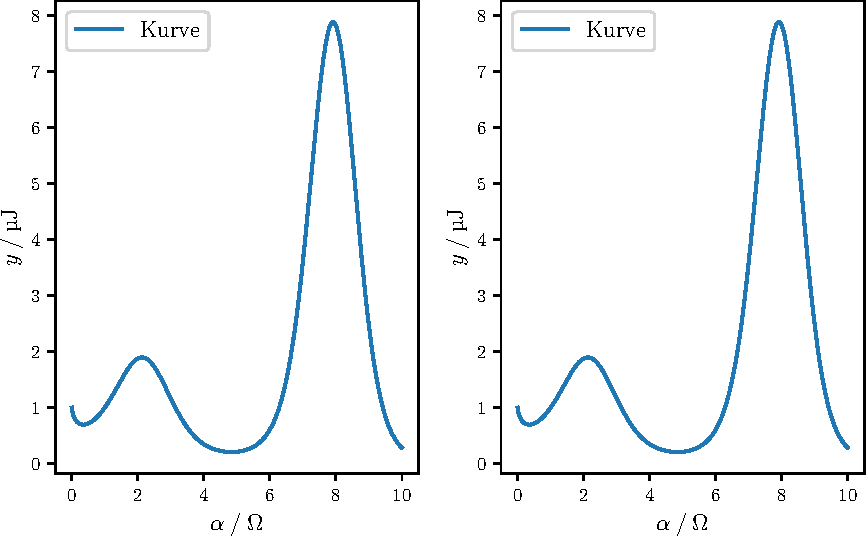
\includegraphics{plot.pdf}
%  \caption{Plot.}
%  \label{fig:plot}
%\end{figure}

%Siehe \autoref{fig:plot}!